\section{The effect of strain in hybrid quantum systems}
The motivation for this project arises due to the interest in coupling RE doped YSO to superconducting resonators using the flip-chip approach~\citep{PhysRevLett.110.157001} or direct metal deposition~\citep{doi:10.1063/1.4894455}. The requirement of cryogenic temperatures for operation is expected to induce strain in the crystal environment. This effect is due to difference in thermal expansion coefficients for the substrates and thus could produce a perturbation of the spin distribution. Similarly, this a concern for donor spins in silicon where superconducting resonators are patterned onto the sample~\citep{doi:10.1063/1.4919761}. 

The expected cause of the observed variation from the bulk properties for nano-fabricated electronic substrates on donor spin doped Si substrates was due to induced electric fields or strain effects~\citep{10.1038/NNANO.2014.211}. Investigation of resonance shifts of three aluminum superconducting resonators pattered on the surface of a 700 nm isotropically purified $^{28}$Si substrate with implanted $^{209}$Bi donors~\citep{PhysRevApplied.9.044014}.Electron paramagnetic resonance (EPR) spectroscopy completed on the $\ket{F=4,m_{F}=-4} \leftrightarrow \ket{F=5,m_{F}=-5}$ transition, where $\Delta m_{F} = \pm 1$. This reveals transition peak splitting each with a 100 $\mu$T linewidth compared to single 20 $\mu$ peak measured in the absence of a patterned superconducting resonator as shown in Fig.~\ref{fig:straininducedsplitting}. 


\begin{figure}[h]
\centering
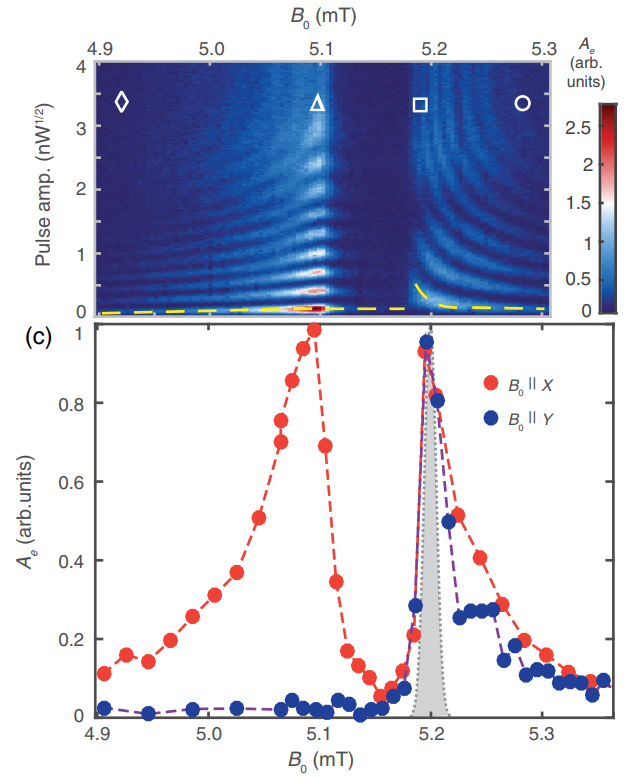
\includegraphics[height=0.45\textwidth,keepaspectratio]{straininducedsplitting}
\caption{\label{fig:straininducedsplitting} The echo signal detected using the Hahn echo sequence for the $\ket{F=4,m_{F}=-4} \leftrightarrow \ket{F=5,m_{F}=-5}$ for $B_{0} \parallel X$ (red) and $B_{0} \parallel Y$ (blue). The grey curve shows the peak transition for the system with no on-chip resonator ~\citep{PhysRevApplied.9.044014}.}
\end{figure}


The low peak observed for  vanishes for $B_{0} \parallel X$ vanishes for $B_{0} \parallel Y$ which is attributed to the condition $\delta B_{1}\perp B_{0}$ for excitation, where $\delta B_{1}$ is the magnetic field vacuum fluctuations in the resonator. Directly under an electrode, of the interdigited LC resonator, dominated by $\delta B_{1Y}$ with contribution of $\delta B_{1Z}$ to the side of the electrode. Therefore, only $\delta B_{1z}$ contributes for $B_{0} \parallel Y$. Further investigation of spin transitions discounts an in-built electric field or magnetic field inhomogeneity as the mechanism for the splitting and broadening of the transition peak. Therefore upon consideration of strain, this mechanism has the ability to modify the electron spin (S=1/2) and nuclear spin (I=9/2) transitions for $^{209}$Bi. Strain can modify the quadrupole interaction, the hyperfine interaction strength $A$ and the electron g-factor.   

The quadrupole interaction arises due to axial symmetry of the nuclear charge distribution where nuclear quadrupole moment $Q$ describes the degree of deformation from spherical charge distribution. The non-spherical nucleus interact with nearby electrons resulting in an electrostatic field gradient $V_{ab}$ at the nucleus where $a$ and $b$ are the local crystal frame principle axes. The Hamiltonian term for the quadrupole interaction is thus:

\begin{equation}
\label{eq:quadropleinteraction}
H_{Q} = \frac{e V_{zz} Q}{4I(2I-1)}\left [3I^{2}_{z}-I^{2}+\eta (I^{2}_{x} - I^{2}_{y} \right ],
\end{equation} 

where the asymmetry parameter is $\eta = (V_{xx}-V_{yy}/V{zz}$ and the electron charge is $e$~\citep{Suits2006}. Ref.~\citep{PhysRevLett.115.057601} demonstrates that the quadrupole interaction can be manipulated by strain applied to Si doped with As$^{+}$ ions using piezo-actuators. The induced strain can be used to tune the nuclear spin properties of As$^{+}$ ions. For the unstrained sample the cubic crystal symmetry cancels out the electric field gradients whilst applying uniaxial strain mimics the effect of strain induced at mK temperatures for substrates with different thermal expansion coefficients and results in a nonzero electric field gradient. 

\begin{figure}[H]
    \centering
    \begin{subfigure}[b]{0.6\textwidth}
        \centering
        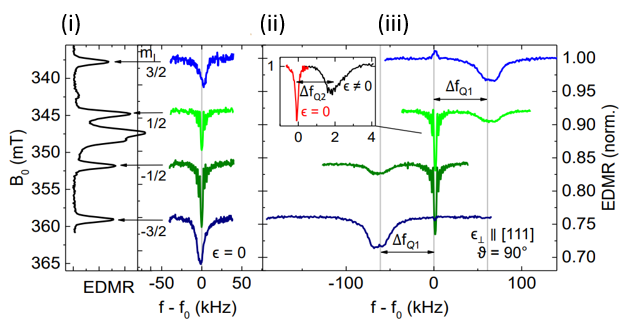
\includegraphics[width=\textwidth]{nuclearshifts}
        \caption{\label{fig:nuclearshifts}(i) electrically detected
magnetic resonance (EDMR) spectrum for As$^{0}$ in Si. (ii) unstrained NMR transitions for As$^{+}$ in Si. (iii) strained NMR transitions for A$^{+}$. The insert shows the $\ket{m_{I}=1/2} \leftrightarrow \ket{-1/2} $ transitions in high-resolution~\citep{PhysRevLett.115.057601}.}
    \end{subfigure}
        \begin{subfigure}[b]{0.6\textwidth}
        \centering
        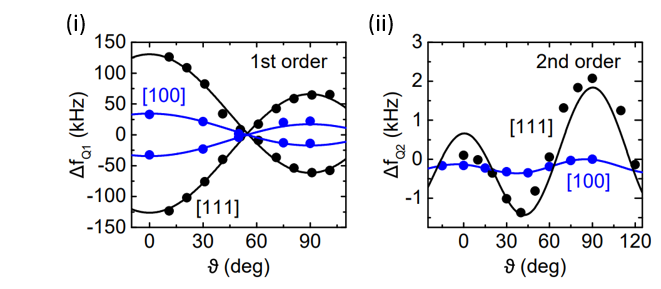
\includegraphics[width=\textwidth]{nuclearshifts2}
        \caption{\label{fig:nuclearshifts2} Angular dependence of (i) first-order and (ii) second-order resonance frequency shifts dependent on the magnetic field orientation where the electric field gradient generated in [111] and [100] crystal directions~\citep{PhysRevLett.115.057601}.}
    \end{subfigure}
    \caption{}
\label{fig:}
\end{figure}

Comparison of the unaxial strain of the order of 10$^{-4}$ and unstrained nuclear magnetic resonance (NMR) spectrum probed using 9.74 GHz resonator is shown in Fig.~\ref{fig:nuclearshifts}. This reveals outer transitions (ie $\ket{m_{I}=3/2} \leftrightarrow \ket{1/2}$ and $\ket{-3/2} \leftrightarrow \ket{-1/2}$ have a resonance shift greater than the resonance linewidth described by the first order frequency shift. Additionally for these transitions asymmetric broadening is observed in absence of the piezo-mechanical strain and is attributed to strain induced by the contact. Conversely only a small second order frequency shift is observed for the sharp $\ket{1/2} \leftrightarrow \ket{-1/2}$ resonance. Further investigation using long rf-pulses as shown in the insert of Fig.~\ref{fig:nuclearshifts} determines that the inner transition is similarly shifted by more than one linewidth but due to the difference in linewidth, between the inner and outer transition, the shift is significantly smaller. Fig.~\ref{fig:nuclearshifts2} presents a characterisation of the resonance shift due to anisotropic electric field gradient as a function of angle $\vartheta$ between magnetic field and strain axis. The quadrupole shift is related to the applied strain through the a tensor $S_{ij}$ with nonzero $S_{11}$ and $S_{44}$ components. However, comparison of $df/dQ$ sensitivity to EPR transitions it is clear the quadrupole interaction is not the origin of the resonance splitting~\citep{PhysRevApplied.9.044014}.

The study of strain induced resonance frequency shifts due to perturbation of the hyperfine coupling of group V donor spins in $^{28}$Si is completed~\citep{doi:10.1063/1.4919761}. The compressive strain is applied using masses placed on top of the sample and is expected to modify the band structure of Si. Thus the valley repopulation model (VRM)~\citep{PhysRev.124.1068} was utilised to understand the effect of Si crystal symmetry breaking which lifts the Si six valley degeneracy. Strain induces mixing of the donor singlet $A_{1}$ ground state and the doublet $E$ excited state. The hyperfine interaction Hamiltonian term is presented in Section.~\ref{sec:hyperfine} where the isotropic hyperfine interaction strength $A$ is given in Eq.~\ref{eq:hyperfinestrength}. The EPR transitions of $^{209}$Bi doped in Si, the sample mount and observed shift in resonance frequency due to small (10$^{-5}$) strain is shown in Fig.~\ref{fig:mansirpaper}. 

\begin{figure}[h]
\centering
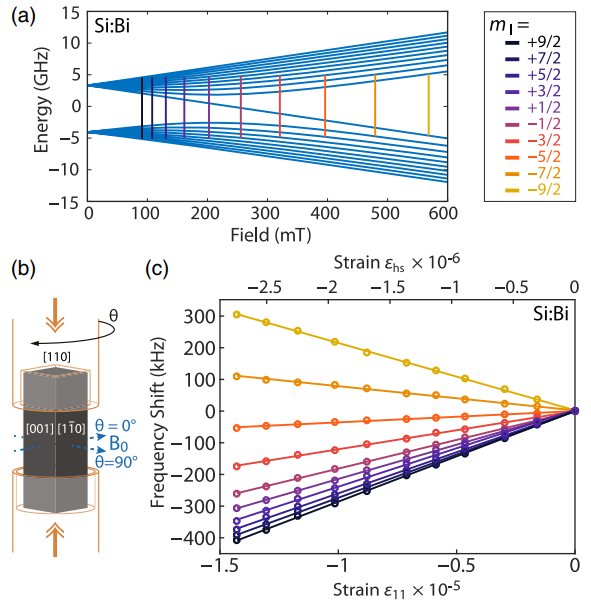
\includegraphics[height=0.45\textwidth,keepaspectratio]{mansirpaper}
\caption{\label{fig:mansirpaper} (a) $^{209}$Bi (S=1/2, I=9/2) doped in Si EPR spectrum. (b) Mechanical strain experimental setup where $\theta$ is orientation of $B_{0}$ with respect to the [001] crystal axis. (c) Observed linear EPR frequency shifts as a function of the strain $\epsilon_{11}$ for $\theta = 30^{\circ}$ ~\citep{doi:10.1063/1.4919761}.}
\end{figure}

The VRM model predicts quadratic shift of $A$ for the application of unaxial strain. However, the observed linear shift is attributed to uniaxial stress applied to the crystal producing three linear strain components, $\epsilon_{11}$, $\epsilon_{22}$ and $\epsilon_{33}$ where the hydrostatic strain mechanism is described as $\epsilon_{hs} = (\epsilon_{11}+\epsilon_{22}+\epsilon_{33}/2$. Comparison of isotropic hyperfine coupling $df/dA$ to the experimentally measured $df/d\epsilon_{11}$ determines the linear strain mechanism dominates. The tight binding (TB) model~\citep{PhysRevB.79.245201} describing the variation of bound states $Bi$ doped Si under strain provides a good agreement for small applied strain with experimentally. The determined relationship $A/A_{0}$ where $A_{0}$ is the unstrained hyperfine interaction strength to second order the strain is:

\begin{equation}
\label{eq:Atermmodel}
A(\bm{\epsilon})/A_{0} = 1+\frac{K}{3}(\epsilon_{xx}+\epsilon_{yy}+\epsilon_{zz})+\frac{L}{2}\left [ (\epsilon_{yy}-epsilon_{zz})^{2}+(\epsilon_{xx}-\epsilon_{zz})^{2}+(\epsilon_{xx}-\epsilon_{yy})^{2}) \right ] +N(\epsilon^{2}_{yz}+\epsilon^{2}_{xz}+\epsilon^{2}_{xy}),
\end{equation} 

where A fit to the TB model obtains K = 29.3, L = -9064 and N = -225. Additionally, investigation the induced anisotropy of the g-tensor for V group donors in Si is fitted to a model developed which contains a VRM term and the spin-orbit coupling term. Applying the model in Eq.~\ref{eq:Atermmodel} to the Si doped As$^{+}$ device with LC resonator pattered on the surface in Ref.~\ref{PhysRevApplied.9.044014} determines $A(\bm{\epsilon}=$ 1MHz for strain of the order of 10$^{-4}$. This results in a resonance shift in agreement with the experimentally measured result of Fig.~\ref{fig:straininducedsplitting}. Therefore the strain induced modification of the $A$ is determined to be the resonance peak splitting mechanism. 


\begin{figure}[h]
\centering
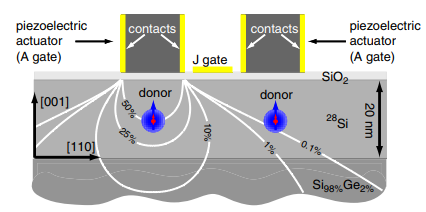
\includegraphics[height=0.45\textwidth,keepaspectratio]{piezoelectric}
\caption{\label{fig:piezoelectric} The schematic of the piezoelectric actuators which can apply strain to the $^{28}$Si substrate in locations of a donor spin. This device tunes the coupling strength between the nuclear and electronic spin of the P donor. The distribution of the out of plane strain is illustrated using isolines is modelled using density function theory calculations. To maximise the effect of the nanoactuators $^{28}$Si is grown on a SiGe substrate ~\citep{PhysRevLett.106.037601}.}
\end{figure}

The applications of the strain induced ability to shift a resonance peak of a spin system by more than a linewidth does not go unnoticed \citep{doi:10.1063/1.4919761,PhysRevApplied.9.044014,PhysRevLett.115.057601}. The scheme to Stark tune the hyperfine interaction of P doped Si using piezoelectric nanoactuators is illustrated in Fig.~\ref{fig:piezoelectric}. This scheme provides a 17 $\mu$T shift of the P hyperfine transitions with a 8 $\mu$T linewidth. Therefore, this device has potential to provide an additional degree of freedom to tune qubits in and out of resonance. Additionally, in Ref.~\citep{PhysRevB.88.064308} applying mechanical stress to a single acceptor in a patterned Si substrate is shown to partially lift the ground state degeneracy. In the presence of strain in addition to the magnetic field the qubit can decoupled to the first order decoupled from the acoustic phonons used to coherently manipulate the state of the qubit.   

The theoretical treatment of the interaction between the applied strain and electron spin of NV centers is presented in Ref.~\citep{PhysRevB.98.075201}. This study suggests that magnetically forbidden transitions, in addition to allowed transition, can be coherently driven using mechanically deforming the crystal at a rate equal to the Rabi frequency. In Ref.~\citep{} the ground state Hamiltonian of the spin system is given as:

\begin{equation}
\label{eq:HamiltonianNV}
H_{NV} = D_{0}S^{2}_{z}+\gamma_{NV}B_{\parallel}S_{z}+\gamma_{NV}B_{\perp}S_{x}+\epsilon_{\perp} \left | \sigma_{x}(S_{x}S_{y}+S_{y}S_{x})+\sigma_{y}(S^{2}_{x}-S^{2}_{y}) \right |, 
\end{equation} 

where $D_{0}$ and $\gamma_{NV}$ is the zero-field splitting and the gyromagnetic ratio, respectively. The degeneracy of the $\ket{m_{s}=0}$ and $\ket{\pm 1}$ is lift by $D_{0}$. The components of the magnetic field are given as $B_{\parallel}$ and $B_{\perp}$ and the components of the electron spin operator as $S_{x},S_{y} and S_{z}$ where z-axis is along the crystal's symmetry axis. Alignment of $B_{\parallel}$ splits the degeneracy of $\ket{+1}$ and $\ket{-1}$. Coherent driving of $\ket{0} \leftrightarrow \ket{\pm 1}$ is achieved by an oscillating $B_{\perp}$ field. The addition of a GHz stress perpendicular to the symmetry axis drives the magnetically forbidden spin transition $\ket{-1} \leftrightarrow \ket{+1}$. Thus addition of mechanical strain enables driving between all the spin states. A bulk acoustic resonator is used to generate the stress resonant with the $\ket{-1} \leftrightarrow \ket{+1}$ transition where the magnetic spin resonance is achieved using an optical detection scheme at room temperature. 

